\documentclass[x11names,compress,mathserif,t]{beamer}
%
\newcommand{\changespace}[1]{\renewcommand{\baselinestretch}{#1}\normalsize}
%
\usepackage{mathptmx}
\usepackage[scaled=.90]{helvet}
\usepackage{courier}
\usepackage[T1]{fontenc}
\usepackage{ulem}
\usepackage[english]{babel}
\usepackage[latin1]{inputenc}
\usepackage{url}
\usepackage{graphicx,color,psfrag}
\usepackage{amsmath,amsfonts,amsthm,amssymb}
\usepackage{subfigure}
\usepackage{multirow}
\usepackage{verbatim}
\usepackage{multimedia}
\usepackage{datetime}
\usepackage{caption}
\usepackage{caption}
\usepackage{ragged2e}
\usepackage{relsize} 
%
\captionsetup{labelformat=empty,labelsep=none}
\setbeamertemplate{caption}[numbered]
\setbeamerfont{caption}{size=\scriptsize}
\setbeamertemplate{itemize item}[triangle] 
%
\definecolor{darkblueone}{rgb}{0.2,0.2,1.0}\newcommand{\darkblue}{\color{darkblueone}}
%
\mode<presentation>
{
  \usetheme{CambridgeUS}
  \beamertemplateballitem
  \useinnertheme[shadow=true]{rounded}
  \setbeamercolor{block title}{fg=white,bg=blue} 
  \setbeamercolor{block body}{fg=black,bg=blue!8!white}
  \setbeamercolor{alerted text}{fg=red, bg=white}
  \setbeamercolor{alerted body}{fg=black,bg=red!8!white}
  \setbeamercolor{palette primary}{fg=black,bg=white} 
  \setbeamercolor{palette secondary}{fg=black,bg=blue!8!white}
  \setbeamercolor{palette tertiary}{bg=blue,fg=white}
  \setbeamercolor{palette quaternary}{fg=black,bg=white}
  \setbeamercolor{title}{bg=blue,fg=white}
  \setbeamercolor{frametitle}{bg=blue!8!white,fg=blue}
  \setbeamercolor{framesubtitle}{bg=blue!8!white,fg=blue}
  \beamertemplatenavigationsymbolsempty
}
%
\pgfdeclareimage[interpolate=true,height=10pt]{oru-logo-small}{figs/oru_logo_small}
\pgfdeclareimage[interpolate=true,height=5pt]{aasslogsmall}{figs/aasslogsmall}
\pgfdeclareimage[interpolate=true,height=69pt]{oru-logo}{figs/roblog_logo}
%
\title[ICRA 2014]{Velvet Fingers: Grasp Planning and Execution for an Underactuated Gripper with Active Surfaces}
%
\author[Robert~Krug]{{\bf R.~Krug}, T.~Stoyanov, M.~Bonilla, V.~Tincani, N.~Vaskevicius,\\ G.~Fantoni, A.~Birk, A.~Lilienthal~and~A.~Bicchi}
%
\institute[AASS]
{
  \hspace{0.4cm}
  \begin{minipage}{0.65\textwidth}
    \vspace{-0.2cm}
    \pgfuseimage{oru-logo}\\
   % \vspace{0.05cm}
  \end{minipage}
  \\
  \changespace{1.005}
  {\footnotesize {\em Mobile Robotics \& Olfaction Lab}}\\
  {\footnotesize {\em Center for Applied Autonomous Sensor Systems (AASS)}}\\
  {\footnotesize {\em \"{O}rebro University, Sweden}}\\
  {\small \url{robert.krug@oru.se}}\\
}
%
\date{}
%
\AtBeginSection[] 
{
  \addtocounter{framenumber}{-1}
  \begin{frame}
    \frametitle{Outline}
    \tableofcontents[currentsection]
  \end{frame}

}
% 
% \beamerdefaultoverlayspecification{<+->}
\begin{document}
\frame{\titlepage}
% ======================================================================================
\frame {
  \frametitle {The RobLog Project}
  \pgfdeclareimage[interpolate=true,width=.5\textwidth]{container}{figs/clutter}
  \begin{columns}
    % 
    \begin{column}[]{0.5\textwidth}
     \vspace{4mm}
      \begin{itemize}
      \item{FP7 European Union project in a logistics setting}
      \item{Autonomous unloading of shipment containers}
      \item{Exploit capabilities of an underactuated gripper with active surfaces}
      \end{itemize}
    \end{column}
    % 
    \begin{column}[]{0.5\textwidth}
      \begin{figure}
        \pgfuseimage{container}
      \end{figure}
    \end{column}
    % 
  \end{columns}
}
% ======================================================================================
\frame {
  \frametitle {The Parcelrobot Platform}
  \pgfdeclareimage[interpolate=true,width=1\textwidth]{parcelbot}{figs/parcel_robot.png}
  \begin{center}
    \pgfuseimage{parcelbot}
  \end{center}
}
% ======================================================================================
\frame {
  \frametitle {Tackled Problem}
  \vspace{2mm}
  \alert{Problem:}
  \begin{itemize}
  \item Find a cost-effective solution for grasping large, simple objects
  \item Reliable grasp planning \& execution in cluttered scenes
  \end{itemize} 
  \vspace{5mm}
  \onslide<2->{
    \alert{Solution:}
    \begin{itemize}
    \item Separate offline grasp synthesis from online motion planning
    \item Incorporate human strategies in the grasp planning
    \item Leverage the capabilities of a simple, underactuated gripper with active surfaces
    \end{itemize}
  }
  % 
}
% ======================================================================================
\section{Concept}
\frame{
  \frametitle{The Velvet Fingers Gripper~\cite{Tinc12}}
  \vspace{2mm}
  \textcolor{blue}{Simplify grasp planning $\rightarrow$ rely on the gripper's capabilities for grasp execution} 
  % 
  \begin{columns}
    \begin{column}[]{0.7\textwidth}
      \begin{itemize}
      \item Two-fingered underactuated structure
      \item Conveyor belts on the finger pads implement Active Surfaces for In-Hand manipulation
      \item One actuated DoF for open/close, two DoF for belt actuation
      \item Proximal phalanges blocked $\rightarrow$ distal phalanges ``wrap around'' the object
      \end{itemize}
    \end{column}
    % 
    \begin{column}[]{0.3\textwidth}
     \begin{figure}
     \centering
      \includegraphics[width=.95\textwidth]{figs/velvet_grasp}
     \end{figure}
    \end{column}
  \end{columns}
}
% ======================================================================================
\frame{
  \frametitle{The Velvet Fingers Gripper~\cite{Tinc12}}
  \vspace{2mm}
  \textcolor{blue}{Simplify grasp planning $\rightarrow$ rely on the gripper's capabilities for grasp execution} 
%
    \begin{center}
      \movie[showcontrols]{\includegraphics[width=.95\textwidth]{figs/velvet}}{velvet.avi}
    \end{center}
}
% ======================================================================================
\frame{
  \frametitle{Contributions}
  \vspace{2mm}
  \textcolor{blue}{Grasp Synthesis framework} 
\begin{itemize}
\item Optimization-based grasp synthesis based on~\cite{Cioc09}
\item Account for strategies observed in humans
\end{itemize}
%
\onslide<2->
%
  \vspace{2mm}
  \textcolor{blue}{In-Hand Manipulation Strategy} 
    \begin{figure}
     \centering
      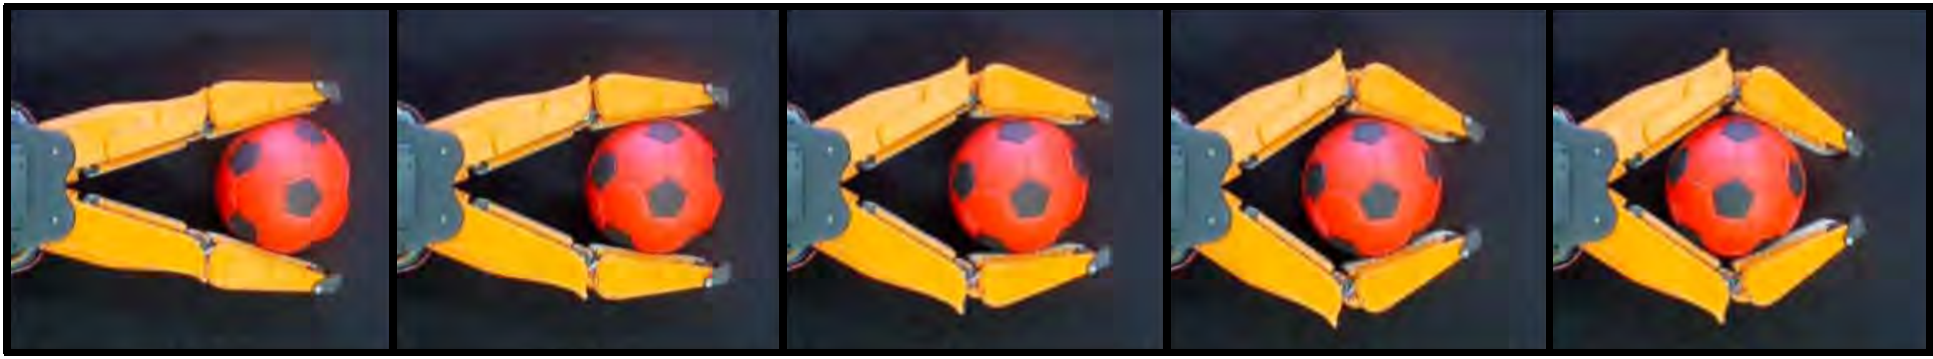
\includegraphics[width=1\textwidth]{figs/pull_in}
     \end{figure}
%
\begin{itemize}
\item In cluttered scenes fingertip grasps are advantageous
\item Increase robustness by ``pulling'' the object in a firm enveloping grasp
\end{itemize}
}
% ======================================================================================
\section{Grasping Pipeline}
\frame{
  \frametitle{Grasping Pipeline}
  \vspace{2mm}
  \textcolor{blue}{Grasp Synthesis is separated from Motion Planning} 
    \begin{figure}
     \centering
      \only<1>{\includegraphics[width=.95\textwidth]{figs/pipeline}}
      \only<2>{\includegraphics[width=.95\textwidth]{figs/pipeline3}}
      \only<3>{\includegraphics[width=.95\textwidth]{figs/pipeline4}}
      \only<4>{\includegraphics[width=.95\textwidth]{figs/pipeline5}}
      \only<5>{\includegraphics[width=.95\textwidth]{figs/pipeline6}}
      \only<6>{\includegraphics[width=.95\textwidth]{figs/pipeline2}}
     \end{figure}
%
\onslide<2->
%
\begin{itemize}
\item<2-> Populate a database with object models (~\cite{Miha13}) \& grasps
\item<3-> Match database objects to the observed scene~\cite{Vask12}
\item<4-> Rank associated grasps with a scoring function~\cite{Bere07}
\item<5-> Execute in a feasible-first manner~\cite{MoveIt} 
\end{itemize}
}
% ======================================================================================
\section{Grasp Synthesis}
\frame{
  \frametitle{Grasp Synthesis}
  \vspace{2mm}
  \textcolor{blue}{Minimize an energy function depending on distance/alignment between object and
    predefined gripper contacts~\cite{Cioc09}}
%
\onslide<2->{
  \begin{columns}
    \begin{column}[]{0.6\textwidth}
      \begin{itemize}
      \item Plan for open/close DoF only
      \item Reference contacts influence grasp type (pinch/envelope)
      \item Impose constraints to account for observed behaviors \ldots
      \item \ldots $e.\,g.$ approach along a surface normal and grasp alignment based on PCA directions
      \end{itemize}
    \end{column}
}
    % 
    \begin{column}[]{0.4\textwidth}
     \begin{figure}
     \centering
      \includegraphics[width=1\textwidth]{figs/preset_contacts}
     \end{figure}
    \end{column}
  \end{columns}


}
% ======================================================================================
\frame{
  \frametitle{Grasp Synthesis}
  \vspace{-4mm}
  \begin{center}
    \movie[showcontrols]{\includegraphics[width=0.85\textwidth]{figs/grasp_planning}}{grasp_planning.avi}
  \end{center}
}
% ======================================================================================
\section{Grasp Execution}
\frame{
 \frametitle{Online Procedure}
 \vspace{2mm}
  \begin{itemize}
  \item<1-> Perform object recognition
  \item<2-> For all detected objects, rank the pre-planned grasps according to a score in the
    current scene
  \begin{align*}
     S&=a_1S_E+a_2S_O\\
         &\\
     a_i &\ldots \mbox{positive weights}\\
     S_E &\ldots \mbox{Energy score}\\
     S_O &\ldots \mbox{Gripper orientation score}
  \end{align*}
  \item<3-> Plan movement trajectories (\cite{MoveIt}) and execute in a feasible-first manner
  \item<4-> \textcolor{blue}{Use a compliant grasp strategy utilizing the active surfaces}
  \end{itemize}
}
% ======================================================================================
\frame{
  \frametitle{Pull-in Grasp Strategy}
  \vspace{2mm}
  \textcolor{blue}{Use current sensing to achieve compliance}  
  % 
  \begin{figure}
    \begin{minipage}[b]{.3\textwidth}
      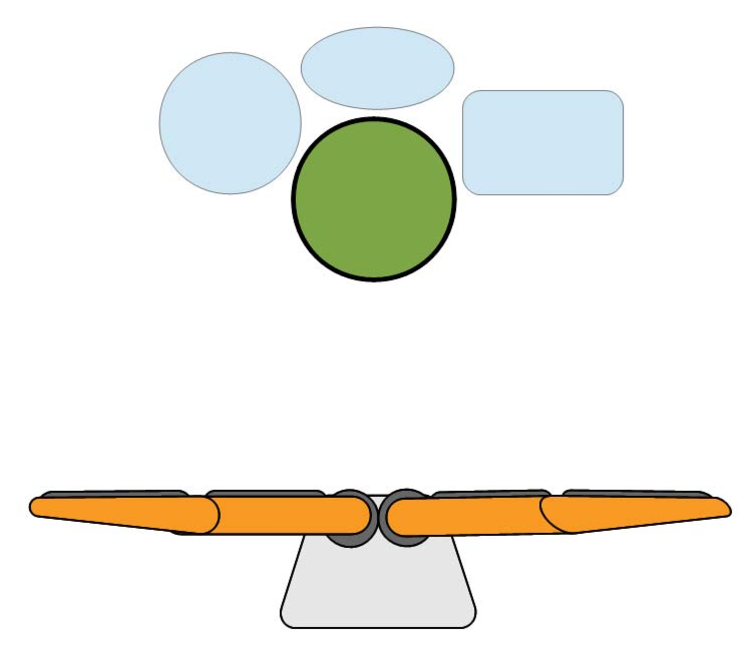
\includegraphics[width = 1\linewidth]{figs/vcg1}
    \end{minipage}
    \begin{minipage}[b]{.3\textwidth}
      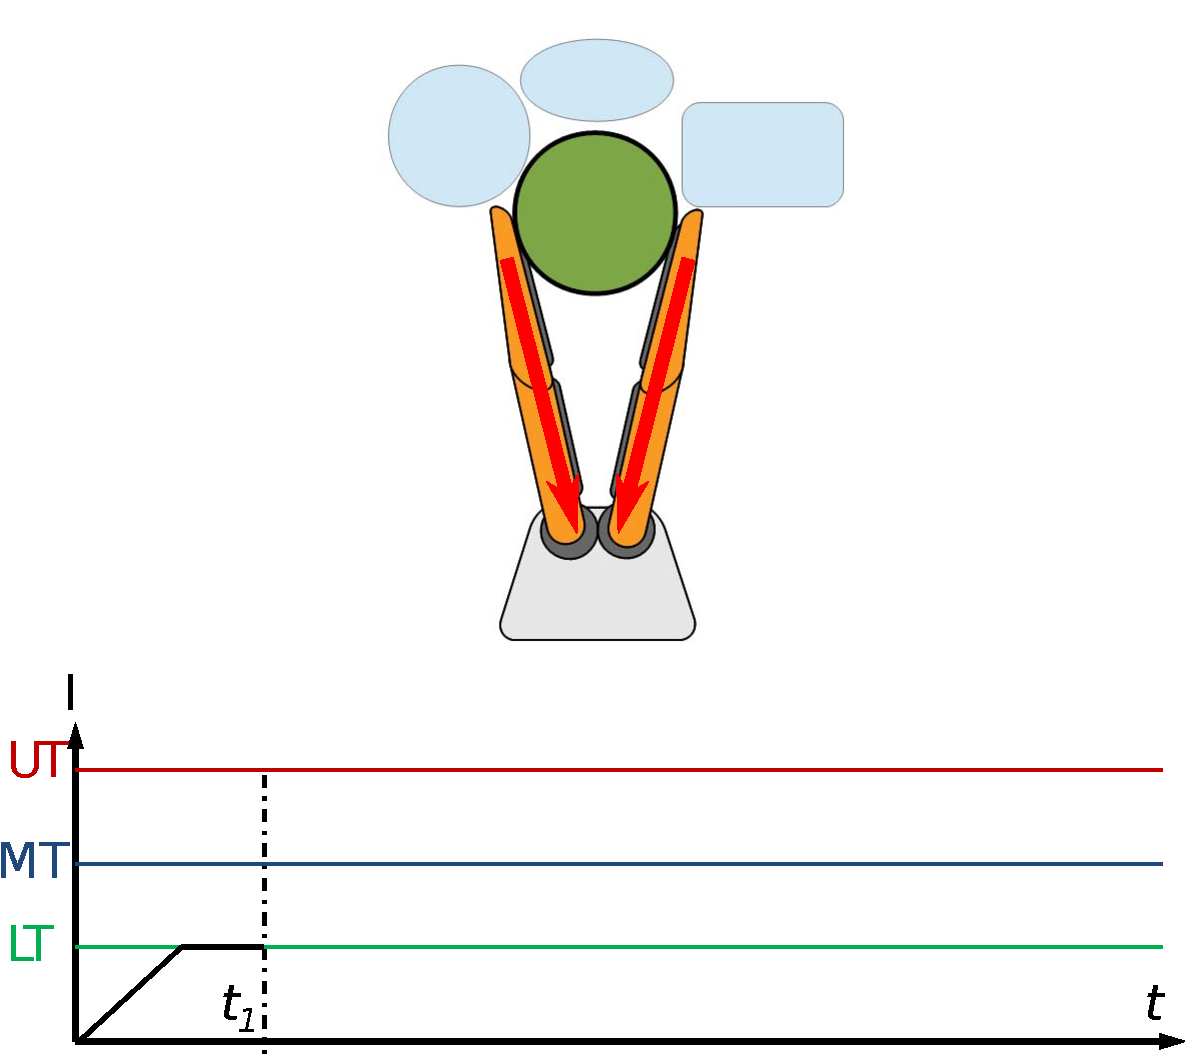
\includegraphics[width = 1\linewidth]{figs/vcg2}
    \end{minipage}
    \begin{minipage}[b]{.3\textwidth}
      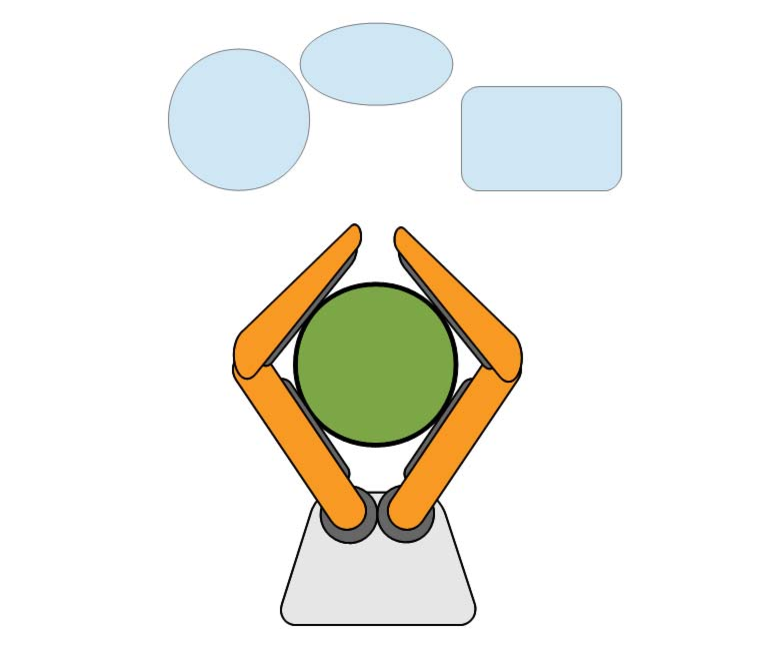
\includegraphics[width = 1\linewidth]{figs/vcg3}
    \end{minipage}
  \end{figure}
%
\begin{itemize}
  \item in cluttered environments many enveloping grasps are infeasible \ldots
  \item \ldots use pinch grasps \& in-hand manipulation
\end{itemize}
}
% ======================================================================================
\frame{
  \frametitle{Test Runs}
  \vspace{-2mm}
  \begin{center}
    \movie[showcontrols]{\includegraphics[width=1\textwidth]{figs/test_runs}}{test_runs.avi}
  \end{center}
}
% ======================================================================================
\section{Contributions \& Outlook}
\frame{
  \frametitle{To sum up \ldots}

  \alert{\textbf{Contributions:}}\\
  \vspace{2mm}
  \begin{itemize}
  \item Optimization-based grasp synthesis \ldots
  \item \ldots incorporating human grasp strategies
  \item In-hand manipulation strategy to increase grasp robustness
  \item \textcolor{blue}{Robust grasp planning \& execution in cluttered scenes}
  \end{itemize}
%
   \vspace{2mm}
  \uncover<2->{ \alert{\textbf{Future work:}}\\}
  \vspace{2mm}
  \begin{itemize}
  \item<2-> Investigate additional use of active surfaces (flipping objects, \ldots)
  \item <2-> Exploitation of additional sensor modalities (torque, tactile)
  \item <2-> \textcolor{blue}{Combined online grasp/motion planning~\cite{Mord12}}
  \end{itemize}
}
% ======================================================================================
\frame{
  \frametitle{That's it \ldots}
  \begin{center}
    \begin{figure}[]
      
\includegraphics[width=0.5\textwidth]{figs/applause}
      % \caption{\textit{State space at time step $k$}}
    \end{figure} 
  \end{center}
}
% ======================================================================================
\section*{References}
{\footnotesize $\;\;$}\\
{\Large {\darkblue References}}
\vspace{0.3cm}
\begin{small}
  \bibliographystyle{apalike}
  \bibliography{References}
\end{small}
\end{document}
% ======================================================================================